% \documentclass[]{article}
\documentclass[conference, onecolumn]{IEEEtran} 

\usepackage[margin=1in]{geometry}
\usepackage{physics}
\usepackage{amsmath}
\usepackage{hyperref}
\usepackage{graphicx}
% \usepackage{multicol}

%opening
\title{MECH 6323 Final Project\\ % come up with something better later
}
\author{Jonas Wagner}
\date{2022-04-10}

\begin{document}

\maketitle

\begin{abstract}
    In this project a model of dynamics of the Autonomous Vehicle (NOVA) will be examined. 
    The NOVA team aims to eventually develop a more fundemental theory-based control strategy, yet there still exists many uncertain and changing parameters that determine the dynamics of the system. 
    In this project a tool to analyze these dynamics, and specifically how we can look at the nonlinearities of the actuators, uncertain physical parameters, and sensor noise/malicious attack will effect the dynamics of the system.

\end{abstract}

% \section{Introduction}

% In this section we reference many self-driving vehicle things... 
% Ideally this intro can be reused in the future for the book chapter.


\section{Underlying System Dynamics}



\begin{figure}%[h]
    \centering
    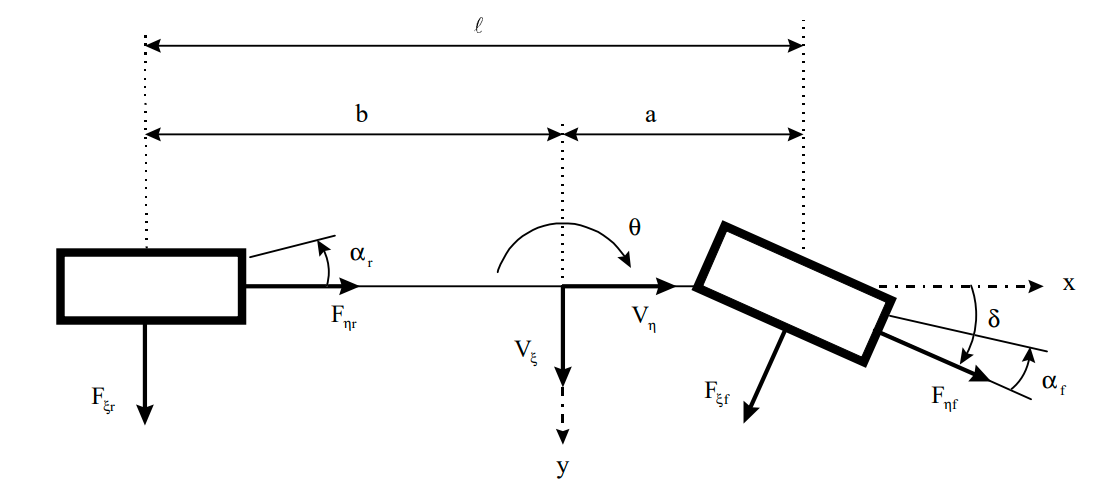
\includegraphics[width=0.5\textwidth]{figs/3dof_model_diag.png}
    \caption{3 DOF Bicycle Model}
    \label{fig:3dof_bike_model}
\end{figure}

\subsection{General Nonlinear Dynamics}
The full nonlinear dynamics for the Bicycle model shown in \figurename{\ref{fig:3dof_bike_model}} are given as: \begin{equation}\begin{cases}
    I \ddot{\theta}     &= a F_{\eta f} \delta + b F_{\zeta f} - b F_{\zeta r}\\
    m (\dot{V_{\zeta}} + V_\eta \dot{\theta}) &= F_{\eta f} \delta + F_{\zeta f} + F_{\zeta r}\\
    m(\dot{V_{\eta}} + V_\zeta \dot{\theta}) &= F_{\eta f} + F_{\eta r} + F_{\zeta f} \delta\\
    \dot{x} &= -V_{\zeta} \sin(\theta) + V_{\eta} \cos(\theta)\\
    \dot{y} &= V_{\eta} \cos(\theta) + V_{\zeta} \sin(\theta)
\end{cases}\label{eq:full_nonlin_eq}\end{equation}
where the global system coordinates are $(x, y, \theta)$, 
longitudinal $(\eta)$ and lateral $(\zeta)$ velocities $(V_\eta, V_\zeta)$,
longitudinal and lateral forces for the front and rear as $(F_{\eta f},F_{\eta r},F_{\zeta f},F_{\zeta r})$,
steering angle of $\delta$, 
and with the following physical parameters that are uncertain:

\begin{table*}[h] \label{tbl:parameters}
    \centering
    \caption{Physical Uncertain Parameters with Nominal Values}
    \begin{tabular}{|r|l|l|}
        \hline
            & Parameter & Nominal\\
        \hline
        $m$ & Vehicle Mass & 1500.0 kg\\
        \hline
        $I$ & Vehicle Yaw Inertia & 12.0 kg m$^2$\\
        \hline
        $a$ & CG Distance to Front Axle & 1.228 m\\
        \hline
        $b$ & CG Distance to Rear Axle & 1.5618 m\\
        \hline
        $c_f$ & Cornering Stiffness of front tire & $0.12 / ^\circ$\\
        \hline
        $c_r$ & Cornering Stiffness of rear tire & $0.16 / ^\circ$\\
        \hline
    \end{tabular}
\end{table*}

There are additional complicated dynamics for how the tire forces are determined based on tire slippage and powertrain dynamics; however this simple plant model takes them as inputs.
Within the actual system actuators are used that control the steering angle and then the force applied to the wheels by friction with the ground is what actually exists as these forces. 
These actuators introduce more complicated dynamics that limit control and also result in even more dependence of uncertain parameters.

\newpage
\subsection{Simulation Formulation}
Within the initial simulations, many assumptions are taken that will be expanded upon when analyzing the robustness to various parameters. 

\subsubsection{State-space Nonlinear Model}
The following is the implementation of the nonlinear dynamics equations \eqref{eq:full_nonlin_eq} in state space with the state vector, $x = [\dot{\theta}, V_\zeta, V_\eta, x, y, \theta]^T$, and input vector $u = [\delta, F_{\eta f}, F_{\eta r}, F_{\zeta f}, F_{\zeta r}]^T$. 
\begin{equation}\begin{cases}
    \dot{x}_1 &= \frac{a F_{\eta,f} \delta + b F_{\zeta,f} - b F_{\zeta,r}}{I}\\
    \dot{x}_2 &= \frac{F_{\eta,f} \delta + F_{\zeta,f} - F_{\zeta,r}}{m} - x_3 x_1\\
    \dot{x}_3 &= \frac{F_{\eta,f} + F_{\eta,r} - F_{\zeta,r}\delta}{m} - x_2 x_1\\
    \dot{x}_4 &= -x_2 \sin(x_6) + x_3 \cos(x_6)\\
    \dot{x}_5 &= x_2 \cos(x_6) + x_3 \sin(x_6)\\
    \dot{x}_6 &= x_1
\end{cases}\end{equation}

\subsubsection{Nominal Nonblinear Model}
Using the Nominal values from \tablename{\ref{tbl:parameters}}, the nominal nonlinear dyanamics are provided as \[
    \left\lbrack \begin{array}{c}
        0.0013\,F_{\eta ,f} -0.0013\,F_{\eta ,r} +0.0010\,F_{\zeta ,f} \,\delta \\
        \text{6.6667e-05}\,F_{\eta ,f} +\text{6.6667e-05}\,F_{\eta ,r} +\text{6.6667e-05}\,F_{\zeta ,f} \,\delta -V_{\eta } \,\dot{\theta} \\
        \text{6.6667e-05}\,F_{\zeta ,f} +\text{6.6667e-05}\,F_{\zeta ,r} -\text{6.6667e-05}\,F_{\eta ,r} \,\delta -V_{\zeta } \,\dot{\theta} \\
        V_{\eta } \,\cos \left(\theta \right)-V_{\zeta } \,\sin \left(\theta \right)\\
        V_{\eta } \,\cos \left(\theta \right)+V_{\zeta } \,\cos \left(\theta \right)\\
        \dot{\theta} 
    \end{array}\right\rbrack
\]

\subsubsection{State-space Linear Model}
Using Jacobian Linearization around a selected equalibrium points/trajectories, we can estimate first-order dynamics near these trajectories by taking the Jacobian of the state-space model with respect to the states and the inputs. 
This results in the dynamic matrices of $A$ and $B$ being defined as follows\[
    A = \eval{\left\lbrack \begin{array}{cccccc}
        0 & 0 & 0 & 0 & 0 & 0\\
        -V_{\eta }  & 0 & -\dot{\theta}  & 0 & 0 & 0\\
        -V_{\zeta }  & -\dot{\theta}  & 0 & 0 & 0 & 0\\
        0 & -\sin \left(\theta \right) & \cos \left(\theta \right) & 0 & 0 & -V_{\zeta } \,\cos \left(\theta \right)-V_{\eta } \,\sin \left(\theta \right)\\
        0 & \cos \left(\theta \right) & \cos \left(\theta \right) & 0 & 0 & -V_{\eta } \,\sin \left(\theta \right)-V_{\zeta } \,\sin \left(\theta \right)\\
        1 & 0 & 0 & 0 & 0 & 0
    \end{array}\right\rbrack}_{x = x_{eq}, u = u_{eq}}
\]\[
    B = \eval{\left\lbrack \begin{array}{ccccc}
        \frac{F_{\zeta ,f} \,a}{\textrm{I}} & \frac{a\,\delta }{\textrm{I}} & 0 & \frac{b}{\textrm{I}} & -\frac{b}{\textrm{I}}\\
        \frac{F_{\zeta ,f} }{m} & \frac{\delta }{m} & 0 & \frac{1}{m} & \frac{1}{m}\\
        -\frac{F_{\eta ,r} }{m} & \frac{1}{m} & \frac{1}{m} & 0 & -\frac{\delta }{m}\\
        0 & 0 & 0 & 0 & 0\\
        0 & 0 & 0 & 0 & 0\\
        0 & 0 & 0 & 0 & 0
    \end{array}\right\rbrack}_{x = x_{eq}, u = u_{eq}}
\]

\subsubsection{Nominal Linear Model}
Linearizing around the arbritrarily chosen $x_{eq} = \mqty[0&0&1&0&0&\frac{\pi}{4}]^T$ and $u_{eq} = \mqty[0.1&1&-1&1&1]^T$, we have the nominal dynamics of $A$ and $B$ being \[
    A = \mqty[
        0       & 0       & 0      & 0 & 0 & 0       \\
        -1.0000 & 0       & 0.1000 & 0 & 0 & 0       \\
        -0.1000 & 0.1000  & 0      & 0 & 0 & 0       \\
        0       & -0.7078 & 0.7064 & 0 & 0 & -0.7785 \\
        0       & 0.7064  & 0.7064 & 0 & 0 & -0.7786 \\
        1.0000  & 0       & 0      & 0 & 0 & 
    ]
\]\[
    B = \mqty[
        0.0010  & 0.0001 & 0      & 0.0013 & -0.0013 \\
        0.0001  & 0.0000 & 0      & 0.0001 & 0.0001  \\
        -0.0001 & 0.0001 & 0.0001 & 0      & -0.0000 \\
        0       & 0      & 0      & 0      & 0       \\
        0       & 0      & 0      & 0      & 0       \\
        0       & 0      & 0      & 0      & 0
    ]
\]

\section{Uncertain Plant Dynamics}
\subsection{Physical Disturbances}
There are many potential physical phenomena that can effect the operation of dynamical systems. 
In the case of a self-driving vehicle, some instances of Direct Disturbances includes disruptions to traction with the ground, such as gravel or wet weather conditions; or similarly, wind resistance and windy weather conditions.

\subsubsection{Tire Slipage}
We will address the actual nonlinear dynamics of tire traction and various modeling methods when discussing the actuator; however, there also exists some general disruptions to tire traction that we can encompass within an additive process noise on the forces excerpted on the wheels:\[
    F_{traction,f} = W_{traction, f} \cdot \qty(V_\zeta \cdot \hat{u}_{\zeta} + V_\eta \cdot \hat{u}_\eta)
\]\[
    F_{traction,r} = W_{traction, r} \cdot \qty(V_\zeta \cdot \hat{u}_{\zeta} + V_\eta \cdot \hat{u}_\eta)
\] Where $W_{traction, f}$ and $W_{traction,r}$ vary greatly depending on the conditions and even a standard filter form is not consistent between conditions.
Although, note that this does make assumptions that the effect on each tire is equivalent relative to the direction the center of mass is moving, not in the direction that the tire specifically is moving.

\subsubsection{Wind Resistance}
Although the NOVA vehicle will be going slow enough that wind resistance is negligible, including it seemed worth while. The effect of wind resistance itself is modeled as two components. 
First, the force due to movement through air proportional to speed is added in the system directly opposite the current direction of movement. 
This is inaccurate in general due to car body shape but this could also be modified to be different weighting from different directions but we will instead just provide for this parameter to vary greatly. \[
    F_{\zeta,w} = k_{\zeta,w} \cdot V_\zeta
\]\[
    F_{\eta,w} = k_{\eta,w} \cdot V_\eta
\]
Second, an additive noise of general stead-state wind either fights against or assists the vehicle. 
The force itself will be applied across the asymmetric body and likely also induce a moment around center of mass, however we will just apply it equally (and opposite when necessary) to each of the wheels to eliminate this. \[
    F_{ws} = W_{ws} \cdot z_{ws} \qty(\cos(\theta - \theta_{ws}) \hat{u}_\eta + \sin(\theta - \theta_{ws}))
\] where $\theta_{ws} \in [0, 2 \pi]$ is the direction that the wind is blowing relative to the global coordinate system defined by the following \[
    \theta_{ws} = W_{w,\theta_{ws}} \cdot z_{w,\theta_{ws}}
\] and both $z_{ws}, z_{w,\theta} \in [0,1]$.
Since wind direction generally changes slowly we will only be looking at lower frequencies so the weighting functions would be of a low-pass filter form: \[
    W_{ws} = \frac{-k_{ws}}{\tau_{ws} s + 1}
\] \[
    W_{w,\theta} = \frac{2\pi}{\tau_{w,\theta} s + 1}
\] where $k_{ws}$ is a selected gain and $\tau_{ws}, \tau_{w,\theta}$ are time constants for the crossover frequency.

Although initially implemented, both of these forms of physical disturbances were left out for simplicity in the current system.

\newpage
\subsection{Nonlinear Actuators}
An important thing this project seeked understand was how the nonlinearities and unknowns within real-life systems will impact performance and robustness of said systems. 
The actuators are a huge part of this difference between ideal theory and what actually happens when implemented, so it is important to account for these things when determining the robustness of systems. 

\subsubsection{Steering and 'Gas'-pedal Response Delays}
Both a human and autonomous driver takes a while to react, while both the steering mechanism and engine/drivetrain also contain delays. 
The driver or self-driving controller will have a delay within the actual system, so a low-pass filter as an actuator will simulate this delayed response by the driver:\[
    W_{driver} = \frac{k_{driver}}{\tau_{driver} s + 1}
\] where $k_{driver}$ is an appropriate gain and $\tau_{driver}$ represents the mean reaction time from decision to actuation for both the steering wheel and gas-pedal.
For steering we would then have:\[
    \delta = W_{driver} \cdot u_{\delta}
\] For the drivetrain there will also be the delay from when the gas-pedal is pressed and when the torque to the wheels applies traction with the ground. \[
    W_{drivetrain} =  \frac{k_{drivetrain}}{\tau_{drivetrain} s + 1}
\] with $k_{drivetrain}$ being the gain from the gas pedal to force on the pavement and $\tau_{drivetrain}$ is the delay it takes for an engine (or non-existent when in a good EV) to ramp up.
We also assume it is only a front-wheel drive vehicle, so only the front wheel will be providing force to move the vehicle, meaning the force that the drivetrain produces will effect the system through $F_{\eta,f}$. 
Therefore, \[
    F_{\eta,f} = W_{drivetrain} \cdot W_{driver} \cdot u_{gas}
\]

\subsubsection{Slip Angle Effects}
The angle of net force excerpted through traction by the wheels is not directly aligned with the direction the wheel is directed. 
These slip angles $\alpha_f$ and $\alpha_r$ are dependent on the current velocity states, $\dot{\theta}, V_{\zeta}, V_{\eta}$, and the steering angle $\delta$.
The front slip angle is calculated as\[
    \alpha_f = \delta - \frac{a \dot{\theta} + V_{\zeta}}{V_{\eta}}
\] and the rear slip angle is \[
    \alpha_r = \frac{b \dot{\theta} - V_{\zeta}}{V_{\eta}}
\]
More complicated methods of modeling this exists, however we will be ignoring things like the saturation regions and maximum traction to have a linear relationship between $\alpha$ and the lateral forces.
The cornering stiffness, $c_f$ and $c_r$, are unknown and vary with conditions. 
The nominal values are shown in \tablename \ \ref{tbl:parameters}. 
The cornering stiffness describes this linear relationship:\[
    F_{\zeta,f} = c_f \cdot \alpha_f
\] \[
    F_{\zeta,r} = c_r \cdot \alpha_r
\]

\newpage
\subsection{Sensors and Measurement Noise}
The biggest challenge that NOVA has been tackling up to now has been developing the localization methods needed to define where the vehicle is at all times. 
This is being done in a variety of ways, all of which are aims of attack we aim to try and exploit in the future. 

\subsubsection{Gyroscope}
First, the gyroscope will measure the rotational velocity of the system which will allow an observer to measure the current state with fairly high accuracy if you sample it well. 
Often software programmers would use this to integrate and find the velocity and position, howowever this isn't really all that useful if you account for the noise at higher frequencies if sampled often.
We can model this measurement as an additive noise that ideally will be eliminated using a good sampling rate.
The gyro measurement output will therefore be:\[
    y_{gyro} = \dot{\theta} + W_{gyro} \cdot z_{gyro}
\] where $z_{gyro} \in [-1,1]$ and noise is modeled by a high-pass filter as\[
    W_{gyro} = \frac{z_{0,gyro} (s + z_{gyro})}{(s+p_{gyro})}
\]

\subsubsection{Spedometer}
The speedometer is just a measurement directly of the Longitudinal Velocity, , and will have a measurement noise that is only really apparent at higher frequencies.
The gyro measurement output will therefore be:\[
    y_{sped} = V_{\eta}  + W_{sped} \cdot z_{sped}, \ z_{sped} \in [-1,1]
\] where $z_{sped} \in [-1,1]$ and noise is modeled by a high-pass filter as\[
    W_{sped} = \frac{z_{0,gyro} (s + z_{sped})}{(s+p_{sped})}
\] 

\subsubsection{GPS}
The GPS system will be used to calculate the global position over a longer period of time for the system. 
Similar to the Gyroscope, the GPS will have error at low ends and isn't going to ever truely be acurate over-time in a real-world situation by itself without other information used by a Kalmen Filter or similar in conjunction with other sensors (such as Lidar) and other localization techniques (which is a big part of what NOVA has been working on this semester) which are also referenced back as the eyeballs. 
We will assume that the sensor error output from the gps will be white noise that is filtered out mostly (because of the way it is averaged and sampled so higher frequencies become less important) except for a region.
\[
    y_{gps, x} = x  + W_{gps} \cdot z_{gps,x}, \ z_{gps,x} \in [-1,1]    
\]\[
    y_{gps, y} = y  + W_{gps} \cdot z_{gps,y}, \ z_{gps,y} \in [-1,1]    
\] where $W_{gps}$ is a bandpass filter:\[
    W_{gps} = \frac{k_{gps} \omega_{gps}^2}{s^2 + 2 \zeta_{gps} \omega_{gps} s + \omega_{gps}^2}
\]

\subsubsection{Eyeballs (Vison \& Loclaization)}
The big thing that isn't included in this entire thing is the actual vision that the vehicle has. Generally this is almost a cheat catch-all of everything since although the sensors will have higher accuracy and ultimately a faster response time, it is the vision that will make things consistent. 
Similarly to the 'driver-delay', we will have a sensing type delay, but all of the information we are able to be aware of is available (although we will have considerably more noise before integrating this information into some sort of Kalmen Filter).\[
    y_{vision} = y + W_{vision} \cdot z_{vision} , \ z_{vision} \in [-1,1]
\] where $W_{gps}$ is a bandpass filter:\[
    W_{vision} = \frac{k_{vision} \omega_{vision}^2}{s^2 + 2 \zeta_{vision} \omega_{vision} s + \omega_{vision}^2}
\]



% \newpage
% \bibliographystyle{ieeetr}
% \bibliography{mybib.bib}


\end{document}
